\documentclass[12pt]{article}
\usepackage{graphicx}
\usepackage{amsmath}
\usepackage{hyperref}
\usepackage{geometry}
\usepackage{float}
\usepackage{subcaption}
\geometry{margin=1in}

\title{Effect of Vehicle Speed on Wireless Communication: \\
Doppler Shift and Rayleigh Fading Analysis}
\author{Hariharan G \\ 1CR23EC069}
\date{}
\begin{document}

\maketitle

\section{Objective}
To investigate the effects of vehicle or receiver speed on wireless communication quality,
this project studies the impact of Doppler shift and Rayleigh fading on the Bit Error Rate (BER)
of Quadrature Phase Shift Keying (QPSK) communication systems.

\section{Problem Statement}

Mobile Wireless communication systems must contend with a time-varying channel caused by 
the relative motion between the transmitter and receiver. This motion introduces a Doppler 
shift in the received signal frequency, and when combined with multipath propagation, gives 
rise to Rayleigh fading, rapid and random fluctuations in the received signal envelope. 
As vehicle speed increases, the channel decorrelates more quickly (shorter
coherence time), which can degrade the reliability of digital communication systems 
that rely on accurate channel knowledge at the receiver.

This project investigates the extent to which vehicle speed affects wireless link 
performance, distinguishing between the fundamental statistical effect of fading 
itself and the practical effect of a receiver's ability (or inability) to track
a fast-changing channel using periodic pilot symbols.

\section{Theory and Background}
\subsection{Doppler Fading}
Doppler Fading is a unique aspect of wireless communication systems. The Doppler shift is a 
fundamental principle related to the electromagnetic radio-wave propagation. The Doppler shift 
associated with an electromagnetic wave is defined as the perceived change in the frequency of 
the wave due to relative motion between the transmitter and receiver. 

The Doppler shift is given by \cite{rappaport}: 
\begin{equation}
    f_d = \frac{v}{\lambda}\cos\theta = \frac{v f_c}{c}\cos\theta
    \label{eq:doppler}
\end{equation}
where $\theta$ is the angle of the line joining the mobile receiver and the base station, $v$ is the
velocity of the mobile receiver, $f_c$ is the carrier frequency, and $c$ is the speed of light.

\subsection{Multipath Propagation and Rayleigh Fading}

In a mobile environment without a dominant line-of-sight path,
the received signal is the sum of many multipath components
arriving from different angles, each with a random amplitude,
phase, and Doppler shift. By the Central Limit Theorem, the
in-phase and quadrature components of the resulting received
signal approach independent, zero-mean Gaussian random
processes for a large number of scatterers \cite{rappaport}. The
envelope of this process, $|h(t)|$, is Rayleigh distributed:

\begin{equation}
    p(r) = \frac{r}{\sigma^2}\exp\left(-\frac{r^2}{2\sigma^2}\right), \quad r \geq 0
    \label{eq:rayleigh_pdf}
\end{equation}

This model, known as \textit{Clarke's reference model}, forms
the theoretical basis for simulating Rayleigh fading channels.


\subsection{Jakes Doppler Power Spectrum}

The multipath components do not arrive with a single Doppler
shift, but rather span the range $[-f_{d,max}, f_{d,max}]$, where $f_{d,max}$ is the maximum 
frequency deviation. The resulting Doppler power spectral density, known as the Jakes
spectrum, is given by:

\begin{equation}
    S(f) = \frac{1}{\pi f_{d,max}\sqrt{1-(f/f_{d,max})^2}}, \quad |f| < f_{d,max}
    \label{eq:jakes_spectrum}
\end{equation}

This characteristic ``bathtub'' shape governs how quickly the
fading channel varies in time: a larger $f_{d,max}$ (higher
speed) corresponds to a wider spectral spread, and therefore a
faster-varying channel envelope.

\subsection{Coherence Time}

The coherence time $T_c$ is a statistical measure of the time
duration over which the channel can be considered approximately
constant. A common approximation is \cite{rappaport}:

\begin{equation}
    T_c \approx \frac{9}{16\pi f_{d,max}}
    \label{eq:coherence_time}
\end{equation}

As speed increases, $f_{d,max}$ increases, and $T_c$ which means that
the channel changes more rapidly, and any channel knowledge obtained by the receiver becomes 
outdated more quickly.

\subsection{Rayleigh Fading Channel Simulation Methods}

Two independent methods were used in this project to generate
a discrete-time, correlated Rayleigh fading channel $h(t)$:

\subsubsection{Smith's Spectral Simulation Method}

This method shapes complex white Gaussian noise in the
frequency domain by the square root of the Jakes power
spectrum (Eq.~\ref{eq:jakes_spectrum}), and then applies an
inverse FFT to obtain a time-domain fading waveform. This
approach is a discrete, computationally efficient realization of
the filtering technique originally proposed by Jakes
\cite{rappaport} and formalized by Smith.


\subsubsection{Zheng--Xiao Sum-of-Sinusoids Method}

This method constructs $h(t)$ directly as a sum of a small
number ($M$) of sinusoids with randomized phase, angle of
arrival, and initial phase parameters \cite{zhengxiao}:

\begin{align}
    X_c(t) &= \frac{2}{\sqrt{M}}\sum_{n=1}^{M}\cos(\psi_n)\cos(w_d t \cos\alpha_n + \phi) \\
    X_s(t) &= \frac{2}{\sqrt{M}}\sum_{n=1}^{M}\sin(\psi_n)\cos(w_d t \cos\alpha_n + \phi)
\end{align}

with $\alpha_n = \frac{2\pi n - \pi + \theta}{4M}$, and $\theta$,
$\phi$, $\psi_n$ independently and uniformly distributed on
$[-\pi,\pi]$. Zheng and Xiao proved that this construction
yields exact second-order statistics (autocorrelation) matching
the theoretical Rayleigh reference model, even for small $M$
(e.g., $M=8$), unlike the original deterministic Jakes
simulator.

\subsection{QPSK Modulation}

Quadrature Phase Shift Keying (QPSK) maps pairs of bits to one
of four constellation points on the unit circle. With
Gray-coded mapping and normalized average symbol energy
$E_s = 1$, the transmitted symbol is:

\begin{equation}
    s = \frac{1}{\sqrt{2}}\left[(2b_1-1) + j(2b_0-1)\right]
    \label{eq:qpsk_symbol}
\end{equation}

where $b_1, b_0 \in \{0,1\}$ are the two bits mapped to that
symbol.

\subsection{Channel Model and Signal-to-Noise Ratio}

The received signal after passing through a flat-fading channel
with additive white Gaussian noise (AWGN) is modeled as:

\begin{equation}
    y(t) = h(t)\,s(t) + n(t)
    \label{eq:channel_model}
\end{equation}

Since QPSK conveys 2 bits per symbol, $E_s = 2E_b$. With
$E_s=1$, the noise spectral density corresponding to a given
$E_b/N_0$ (linear) is:

\begin{equation}
    N_0 = \frac{1}{2(E_b/N_0)}
    \label{eq:n0}
\end{equation}

\subsection{Equalization and Channel State Information (CSI)}

To recover the transmitted symbol, the receiver must undo the
channel's effect, which requires knowledge of $h(t)$ --
referred to as Channel State Information (CSI). Two CSI
scenarios were studied:

\begin{itemize}
    \item \textbf{Perfect CSI}: the receiver has exact,
    instantaneous knowledge of $h(t)$.
    \item \textbf{Estimated CSI}: the receiver estimates $h(t)$
    only at known pilot symbol positions and interpolates
    between them, as is done in practical systems.
\end{itemize}

For equalization the Zero-Forcing method was implemented:

\begin{align}
    \text{Zero-Forcing (ZF):} \quad & \hat{s} = \frac{y}{h} \label{eq:zf}\\
\end{align}

ZF perfectly inverts the channel but amplifies noise
significantly when $|h|$ is small (deep fade).

\subsection{Theoretical QPSK BER over Rayleigh Fading}

For QPSK with coherent detection over a Rayleigh fading channel
under perfect CSI, the average BER as a function of average
$E_b/N_0$ ($\gamma$) has the expression
\cite{simon_alouini}:

\begin{equation}
    P_b = \frac{1}{2}\left(1 - \sqrt{\frac{\gamma}{1+\gamma}}\right)
    \label{eq:theoretical_ber}
\end{equation}

This expression is used throughout this report as the reference
for validating simulation results.


\section{Simulation Methodology}
\subsection{Software Used}

All simulations were implemented in \textbf{Python}, using the \textit{NumPy}  
library for numerical computations, \textit{SciPy} for channel interpolation, and 
\textit{Matplotlib} for visualization. 

\subsection{Simulation Parameters}

\begin{table}[htbp]
\centering
\begin{tabular}{ll}
\hline
\textbf{Parameter} & \textbf{Value} \\
\hline
Carrier frequency, $f_c$        & 2 GHz \\
Vehicle speeds                  & 20, 60, 120 kmph \\
Symbol rate, $f_s$               & 10 kHz \\
Modulation                      & QPSK \\
Number of bits simulated        & $10^5$--$10^6$ \\
$E_b/N_0$ sweep range            & 0--25 dB (2 dB steps) \\
Zheng--Xiao sinusoid count, $M$  & 12 \\
Pilot spacing (sparse case)     & 20 symbols \\
Pilot spacing (matched case)    & 8 symbols \\
Channel estimation method       & Linear interpolation between pilots \\
Equalization methods            & Zero-Forcing, MMSE \\
\hline
\end{tabular}
\caption{Simulation parameters used throughout this project.}
\label{tab:params}
\end{table}

Symbol rate of 10~kHz was chosen to balance computation speed and simulation
artifacts due to the Nyquist limit.

\subsection{Simulation Flow}

The simulation proceeds through following stages for each speed and $E_b/N_0$ value:

\begin{enumerate}
    \item Generate a random bit-stream and modulate it into QPSK symbols (Eq. ~\ref{eq:qpsk_symbol}))
    \item Insert known pilot symbols at fixed intervals into the transmitted symbol bit-stream
    \item Generate the Rayleigh fading channel $h(t)$ for the given speed, using either Smith's spectral method or Zheng--Xiao sum-of sinusoids method.
    \item Pass the transmitted signal through the fading channel and add AWGN corresponding to the target $E_b/N_0$ (Eq.~\ref{eq:channel_model}).
    \item Estimate the channel at the receiver by interpolating between the pilot symbols.
    \item Equalize the received signal using Zero-Forcing (Eqs.~\ref{eq:zf}).
    \item Perform threshold-based QPSK demodulation and compute the Bit Error Rate by comparing recovered bits against the original bitstream.
\end{enumerate}

Figure~\ref{fig:blockdiagram} shows the simulation flow.

\begin{figure}
    \centering
    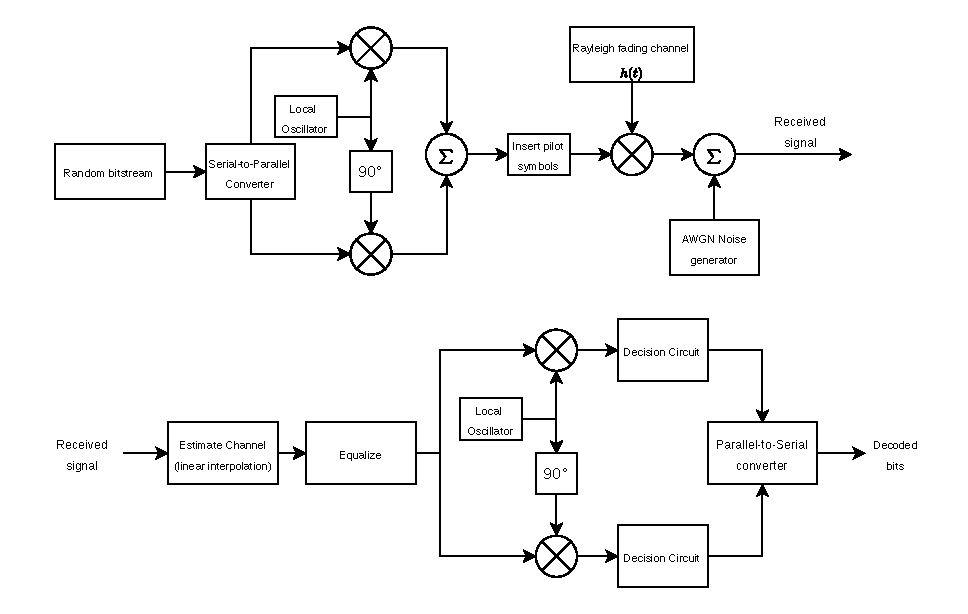
\includegraphics[width=0.75\textwidth]{./diagrams/blockdiagram.pdf}
    \caption{Block diagram of simulation flow.}
    \label{fig:blockdiagram}
\end{figure}

\section{Discussion}
\subsection{Graphs and Interpretations}
\subsubsection{Doppler Spectrum and Channel Gain}

Figure~\ref{fig:doppler_spectrum} shows the Jakes Doppler power spectrum (Eq.~\ref{eq:jakes_spectrum}) for the three simulated speeds. As expected,
higher speeds produce a wider spectral spread, with the characteristic ``bathtub'' sharply cutting off at $\pm f_{d,max}$.

\begin{figure}[htbp]
    \centering
    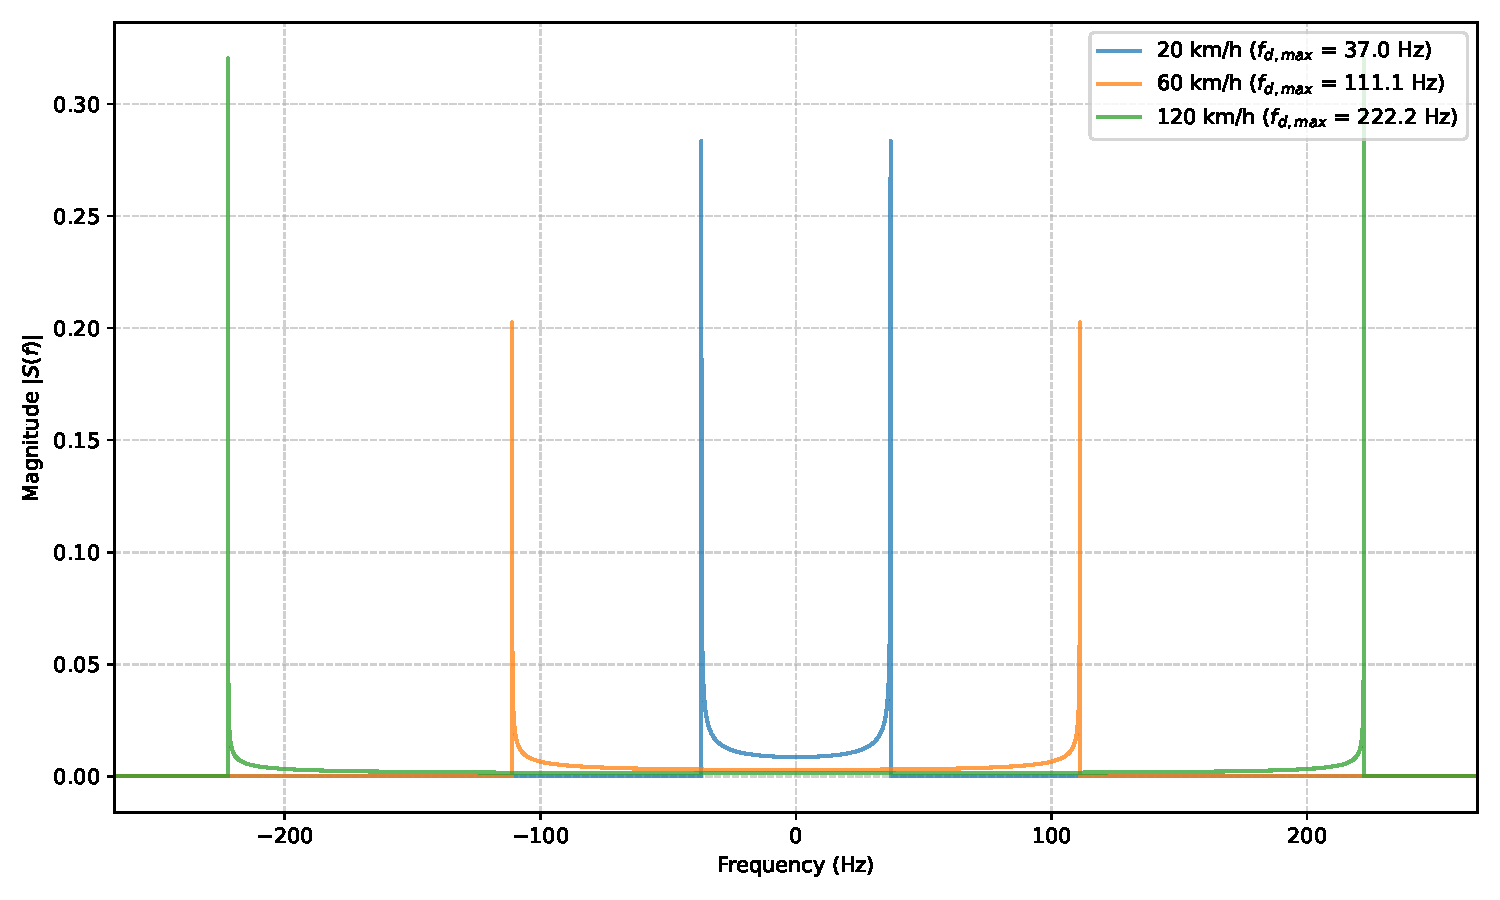
\includegraphics[width=0.75\textwidth]{./diagrams/doppler_spectrum.pdf}
    \caption{Jakes Doppler Spectrum at 20, 60 and 120 kmph}
    \label{fig:doppler_spectrum}
\end{figure}

Figure~\ref{fig:channel_gain} shows the time-domain fading
envelope $|h(t)|$ generated using Smith's spectral method. Faster speeds correspond to more rapid fluctuation of this 
envelope, reflecting the shorter coherence time associated with higher Doppler spread.

\begin{figure}[htbp]
\centering
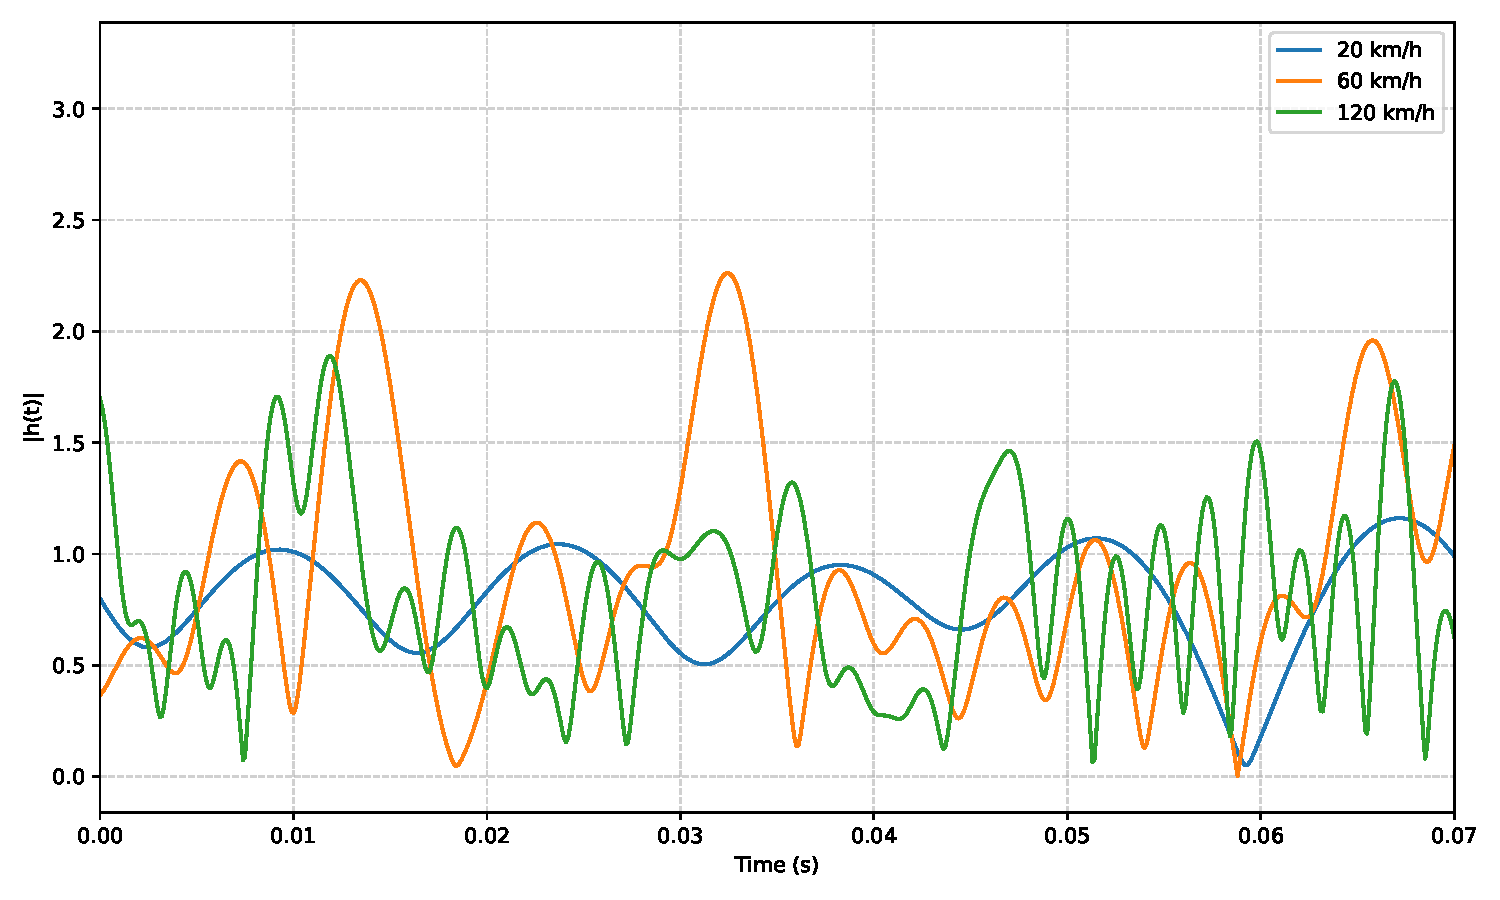
\includegraphics[width=0.75\textwidth]{./diagrams/channel_gain.pdf}
\caption{Rayleigh fading envelope $|h(t)|$ vs.\ time at 20, 60,
and 120 kmph.}
\label{fig:channel_gain}
\end{figure}

The statistical validity of the simulated channel was confirmed by comparing the histogram of $|h(t)|$ against the theoretical
Rayleigh probability density function (Eq.~\ref{eq:rayleigh_pdf}), which showed close agreement for both the Smith and Zheng--Xiao
generation methods.

\subsubsection{BER under Perfect Channel State Information}

Figure~\ref{fig:ber_perfect_csi} shows simulated BER vs.\
$E_b/N_0$ under Rayleigh fading, assuming the receiver has
perfect, instantaneous knowledge of $h(t)$. All three speeds
produce nearly identical BER curves, and both independent
fading generation methods (Smith's and Zheng--Xiao) agree
closely with the theoretical Rayleigh-fading QPSK BER formula
(Eq.~\ref{eq:theoretical_ber}).

\begin{figure}[htbp]
\centering
\begin{subfigure}[b]{0.48\textwidth}
    \centering
    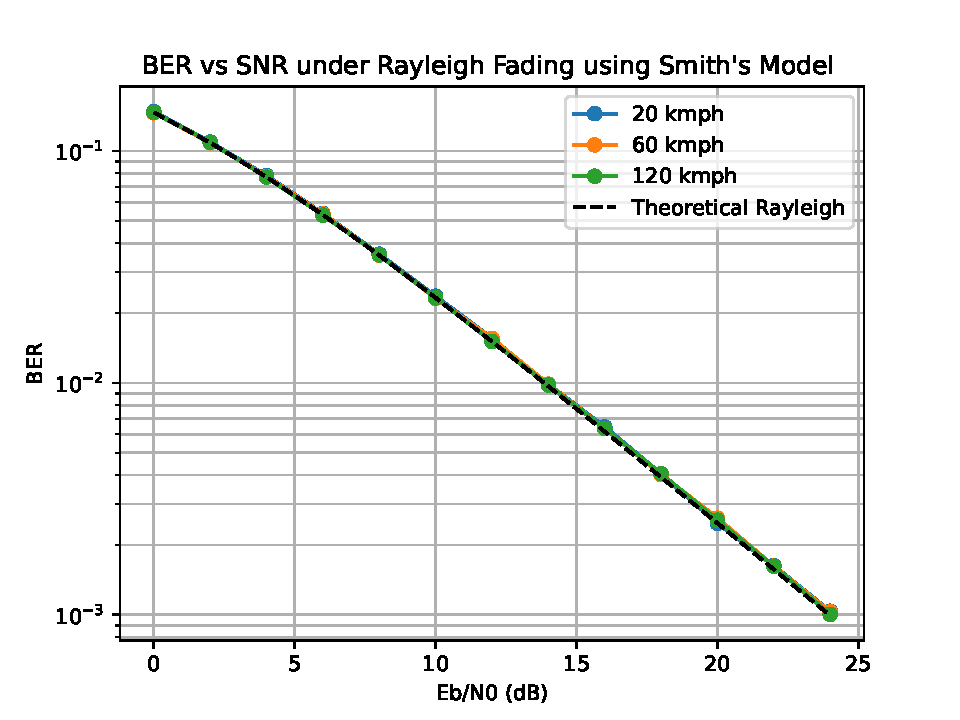
\includegraphics[width=\linewidth]{./diagrams/ber_perfect_csi.pdf}
    \caption{Simulated using Smith's method}
    \label{fig:ber_perfect_csi_jk}
\end{subfigure}
\hfill
\begin{subfigure}[b]{0.48\textwidth}
    \centering
    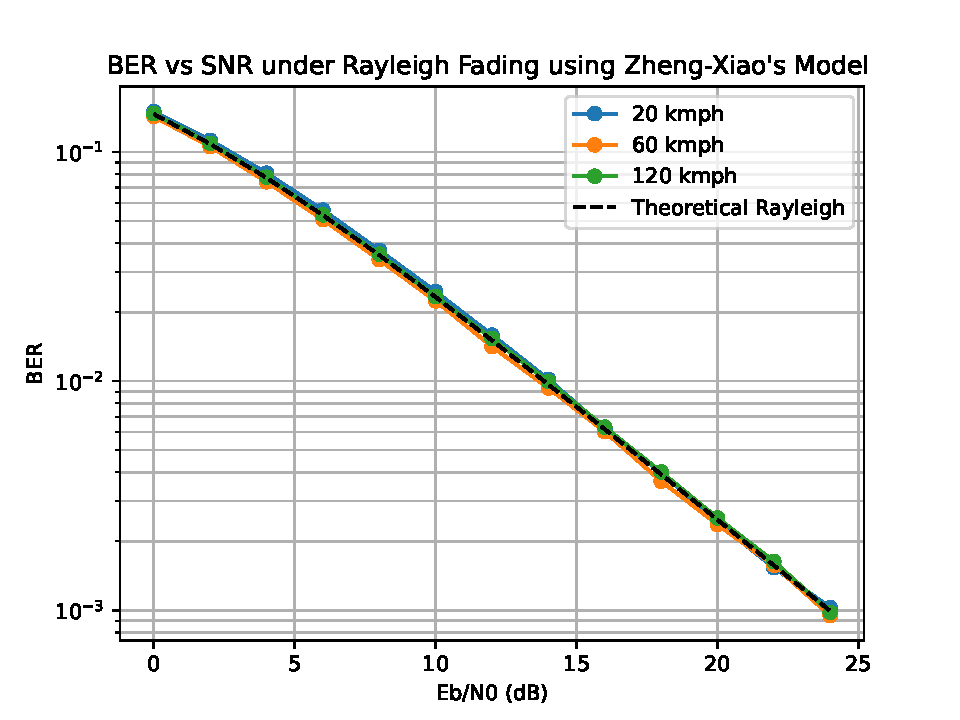
\includegraphics[width=\linewidth]{./diagrams/ber_perfect_csi_zx.pdf}
    \caption{Simulated using Zheng-Xiao's method}
    \label{fig:ber_perfect_csi_zx}
\end{subfigure}
\caption{Simulated BER vs.\ $E_b/N_0$ under perfect CSI for 20, 60, and 120 kmph, compared against the theoretical Rayleigh
BER curve.}
\label{fig:ber_perfect_csi}
\end{figure}

Since the receiver has perfect Channel State Information (CSI) at every instant of time, it instantly knows
the exact channel state for every symbol and cancels it out completely.

\subsubsection{BER under Realistic Pilot-Based Channel Estimation}

Figure~\ref{fig:ber_sparse_pilot} shows BER vs.\ $E_b/N_0$ when the receiver instead estimates $h(t)$ via linear interpolation
between pilot symbols spaced 20 symbols apart. Here, a clear speed-dependent gap emerges: 120~kmph performs consistently
worse than 60~kmph, which performs worse than 20~kmph, with the gap widening as $E_b/N_0$ increases.

\begin{figure}[htbp]
\centering
\begin{subfigure}[b]{0.48\textwidth}
    \centering
    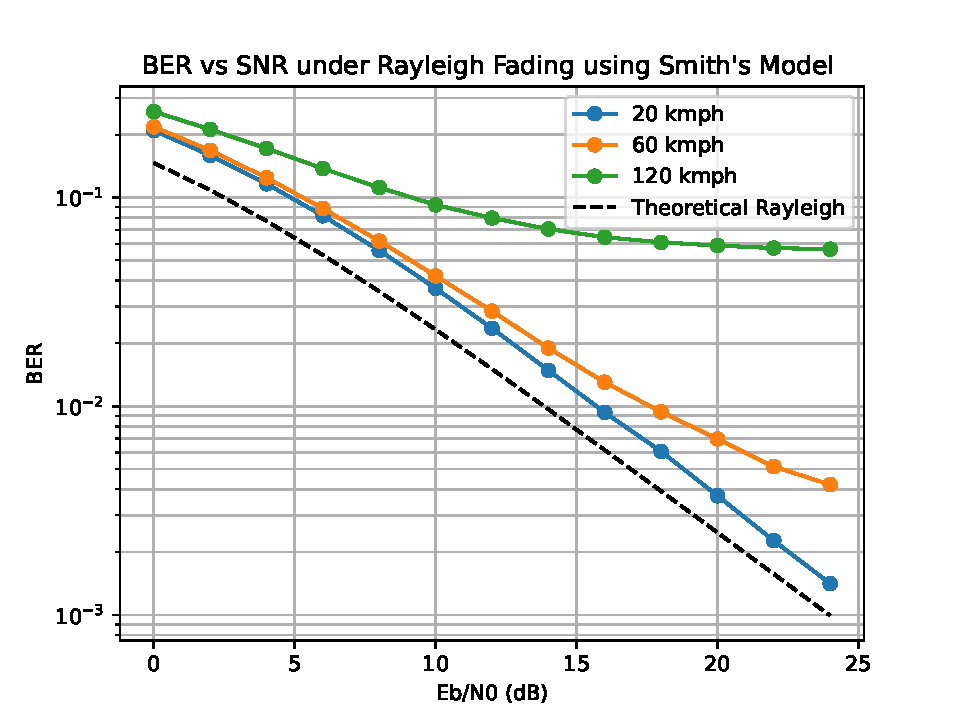
\includegraphics[width=\linewidth]{./diagrams/ber_sparse_pilot.pdf}
    \caption{Simulated using Smith's method}
    \label{fig:ber_sparse_pilot_jk}
\end{subfigure}
\hfill
\begin{subfigure}[b]{0.48\textwidth}
    \centering
    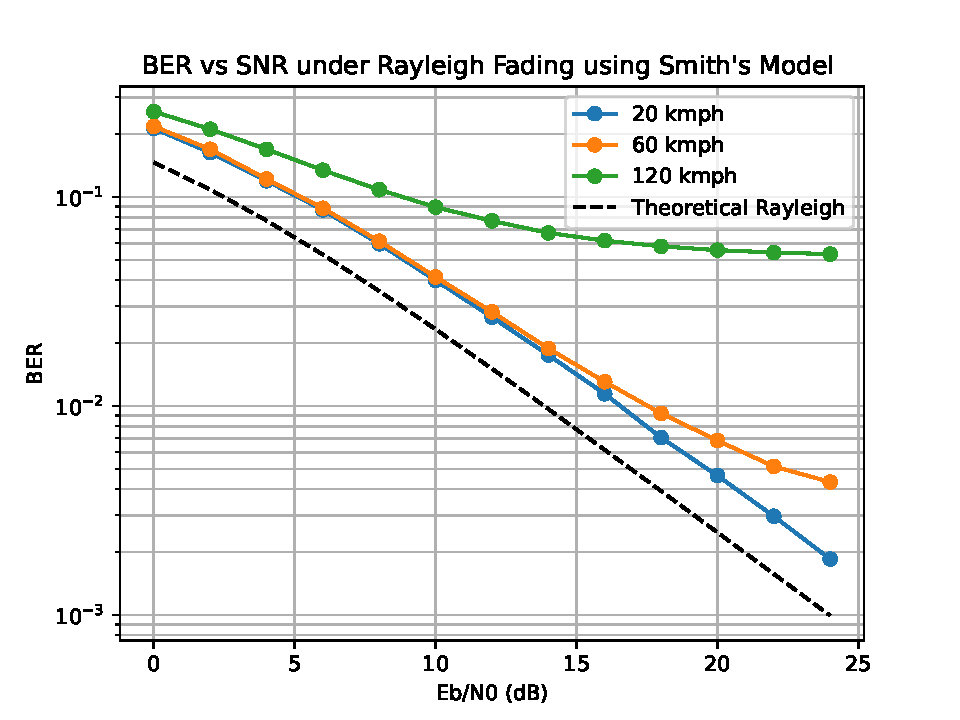
\includegraphics[width=\linewidth]{./diagrams/ber_sparse_pilot_zx.pdf}
    \caption{Simulated using Zheng-Xiao's method}
    \label{fig:ber_sparse_pilot_zx}
\end{subfigure}
\caption{Simulated BER vs.\ $E_b/N_0$ with pilot-based channel
estimation (pilot spacing = 20 symbols), for 20, 60, and 120
kmph.}
\label{fig:ber_sparse_pilot}
\end{figure}

At low SNRs, additive noise is the main cause of bit errors, so speed makes little difference and the curves stay close together.

At high SNRs, noise drops off and channel estimation error takes over as the main bottleneck. Because the channel changes faster at higher 
speeds, a fixed pilot spacing cannot keep up with rapid fluctuations. This creates an error floor where BER flattens out and stops improving, 
making the gap between speeds much wider which is clearly visible at 120 kmph.

\subsubsection{Effect of Pilot Spacing}

The pilot spacing was reduced to 8 symbols -- matching the calculated coherence time at 120~kmph
(Eq.~\ref{eq:coherence_time}). Figure~\ref{fig:ber_matched_pilot} shows that under this denser pilot spacing, the BER gap between
speeds nearly disappears, with all three curves converging close to the perfect-CSI result.


\begin{figure}[htbp]
\centering
\begin{subfigure}[b]{0.48\textwidth}
    \centering
    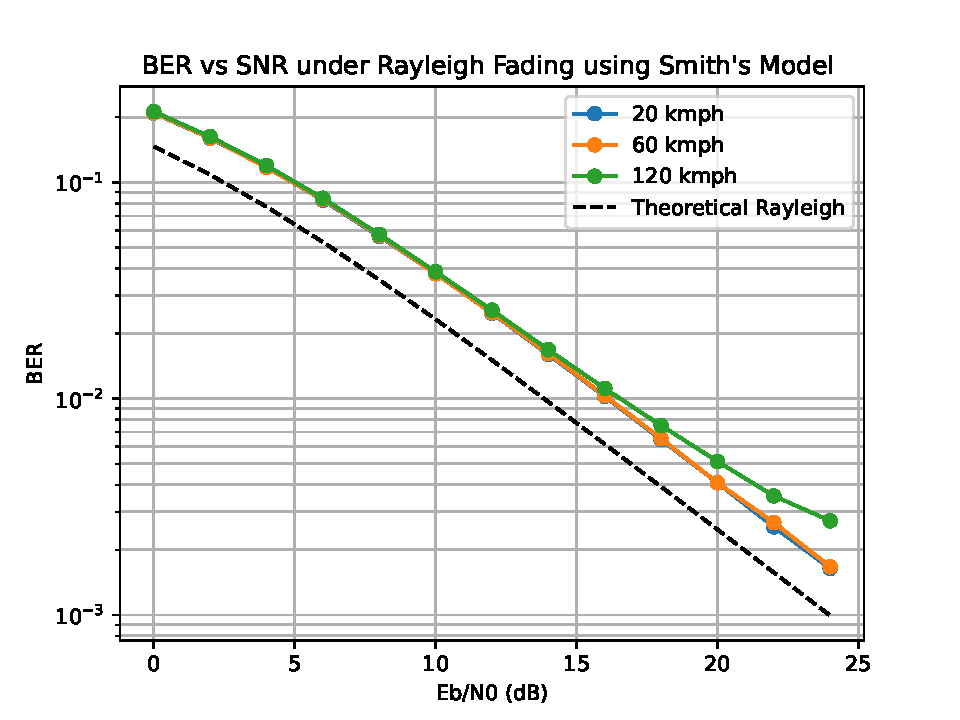
\includegraphics[width=\linewidth]{./diagrams/ber_matched_pilot.pdf}
    \caption{Simulated using Smith's method}
    \label{fig:ber_matched_pilot_jk}
\end{subfigure}
\hfill
\begin{subfigure}[b]{0.48\textwidth}
    \centering
    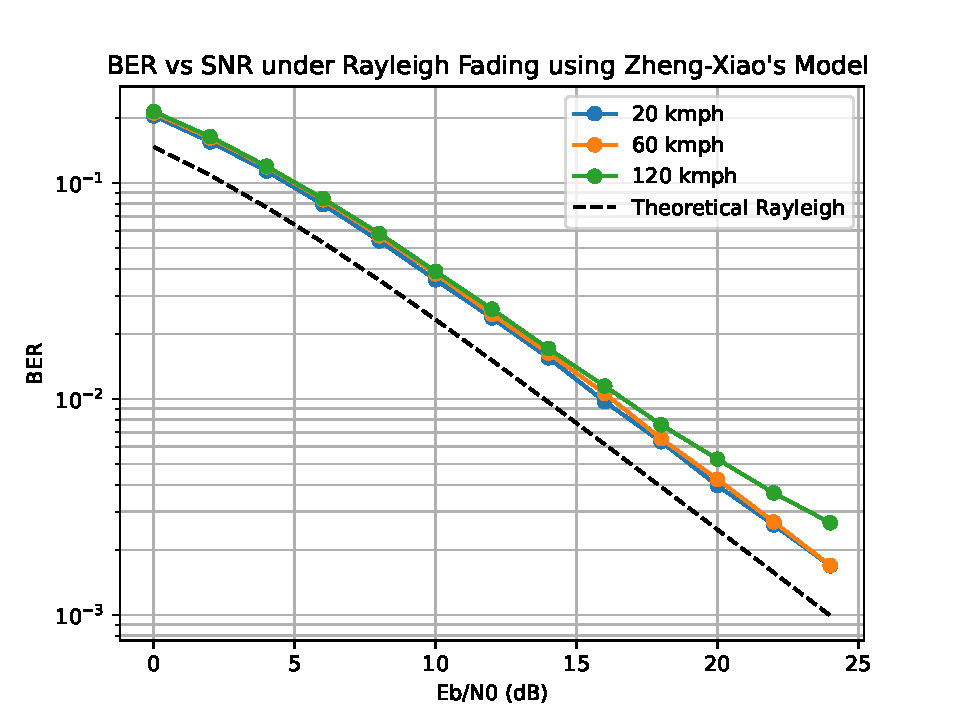
\includegraphics[width=\linewidth]{./diagrams/ber_matched_pilot_zx.pdf} % Replace with your image filename
    \caption{Simulated using Zheng-Xiao method.}
    \label{fig:ber_matched_pilot_zx}
\end{subfigure}

\caption{Simulated BER vs.\ $E_b/N_0$ with pilot spacing reduced to 8 symbols
    (matched to the 120 kmph coherence time), for 20, 60, and 120 kmph.}
\label{fig:ber_matched_pilot}
\end{figure}

This result provides direct, quantitative simulation evidence
that speed-dependent BER degradation is driven by
\emph{channel estimation staleness} relative to coherence time,
rather than by the fading process itself.

\section{Conclusion}
This project investigated the impact of vehicle speed on wireless communication 
quality by simulating Doppler shift, Rayleigh fading, and QPSK link performance 
using two channel generation techniques: Smith’s spectral shaping method and the 
Zheng–Xiao sum-of-sinusoids method. The findings indicate that signal degradation 
at higher speeds is not driven by fading statistics alone, but by practical 
channel estimation limits. As vehicle speed increases, the channel's coherence 
time decreases, causing pilot-based estimates to become stale more quickly. 
This was demonstrated by observing a significant BER gap between speeds when 
pilot spacing exceeded the coherence time, and showing that this gap closed when 
pilot spacing was reduced to match the shortened coherence time at high speeds.

Therefore, at lower speeds the longer coherence time allows pilot-based 
interpolation to track the channel more accurately which directly results in
better performance. At higher speeds, however, the channel changes faster than 
the receiver can estimate using the pilot-based estimation leading to call drops 
and reduced communication quality. For this reason, modern cellular standards 
adaptively scale reference signal (pilot) density for high-mobility 
user equipment.

Overall, this project confirmed theoretical Rayleigh fading models, 
explained why vehicle speed degrades wireless signal quality.


\begin{thebibliography}{9}

\bibitem{rappaport}
T. S. Rappaport,
\textit{Wireless Communications: Principles and Practice},
2nd ed. Upper Saddle River, NJ: Prentice Hall, 2002.

\bibitem{zhengxiao}
Y. R. Zheng and C. Xiao,
``Simulation Models With Correct Statistical Properties for
Rayleigh Fading Channels,''
\textit{IEEE Transactions on Communications}, vol. 51, no. 6,
pp. 920--928, Jun. 2003.

\bibitem{simon_alouini}
M. K. Simon and M.-S. Alouini,
\textit{Digital Communication over Fading Channels},
2nd ed. Hoboken, NJ: Wiley-Interscience, 2005.

\end{thebibliography}

\end{document}